\documentclass[11pt,preprint, authoryear]{elsarticle}

\usepackage{lmodern}
%%%% My spacing
\usepackage{setspace}
\setstretch{1.2}
\DeclareMathSizes{12}{14}{10}{10}

% Wrap around which gives all figures included the [H] command, or places it "here". This can be tedious to code in Rmarkdown.
\usepackage{float}
\let\origfigure\figure
\let\endorigfigure\endfigure
\renewenvironment{figure}[1][2] {
    \expandafter\origfigure\expandafter[H]
} {
    \endorigfigure
}

\let\origtable\table
\let\endorigtable\endtable
\renewenvironment{table}[1][2] {
    \expandafter\origtable\expandafter[H]
} {
    \endorigtable
}


\usepackage{ifxetex,ifluatex}
\usepackage{fixltx2e} % provides \textsubscript
\ifnum 0\ifxetex 1\fi\ifluatex 1\fi=0 % if pdftex
  \usepackage[T1]{fontenc}
  \usepackage[utf8]{inputenc}
\else % if luatex or xelatex
  \ifxetex
    \usepackage{mathspec}
    \usepackage{xltxtra,xunicode}
  \else
    \usepackage{fontspec}
  \fi
  \defaultfontfeatures{Mapping=tex-text,Scale=MatchLowercase}
  \newcommand{\euro}{€}
\fi

\usepackage{amssymb, amsmath, amsthm, amsfonts}

\def\bibsection{\section*{References}} %%% Make "References" appear before bibliography


\usepackage[round]{natbib}

\usepackage{longtable}
\usepackage[margin=2.3cm,bottom=2cm,top=2.5cm, includefoot]{geometry}
\usepackage{fancyhdr}
\usepackage[bottom, hang, flushmargin]{footmisc}
\usepackage{graphicx}
\numberwithin{equation}{section}
\numberwithin{figure}{section}
\numberwithin{table}{section}
\setlength{\parindent}{0cm}
\setlength{\parskip}{1.3ex plus 0.5ex minus 0.3ex}
\usepackage{textcomp}
\renewcommand{\headrulewidth}{0.2pt}
\renewcommand{\footrulewidth}{0.3pt}

\usepackage{array}
\newcolumntype{x}[1]{>{\centering\arraybackslash\hspace{0pt}}p{#1}}

%%%%  Remove the "preprint submitted to" part. Don't worry about this either, it just looks better without it:
\makeatletter
\def\ps@pprintTitle{%
  \let\@oddhead\@empty
  \let\@evenhead\@empty
  \let\@oddfoot\@empty
  \let\@evenfoot\@oddfoot
}
\makeatother

 \def\tightlist{} % This allows for subbullets!

\usepackage{hyperref}
\hypersetup{breaklinks=true,
            bookmarks=true,
            colorlinks=true,
            citecolor=blue,
            urlcolor=blue,
            linkcolor=blue,
            pdfborder={0 0 0}}


% The following packages allow huxtable to work:
\usepackage{siunitx}
\usepackage{multirow}
\usepackage{hhline}
\usepackage{calc}
\usepackage{tabularx}
\usepackage{booktabs}
\usepackage{caption}


\newenvironment{columns}[1][]{}{}

\newenvironment{column}[1]{\begin{minipage}{#1}\ignorespaces}{%
\end{minipage}
\ifhmode\unskip\fi
\aftergroup\useignorespacesandallpars}

\def\useignorespacesandallpars#1\ignorespaces\fi{%
#1\fi\ignorespacesandallpars}

\makeatletter
\def\ignorespacesandallpars{%
  \@ifnextchar\par
    {\expandafter\ignorespacesandallpars\@gobble}%
    {}%
}
\makeatother

\newenvironment{CSLReferences}[2]{%
}

\urlstyle{same}  % don't use monospace font for urls
\setlength{\parindent}{0pt}
\setlength{\parskip}{6pt plus 2pt minus 1pt}
\setlength{\emergencystretch}{3em}  % prevent overfull lines
\setcounter{secnumdepth}{5}

%%% Use protect on footnotes to avoid problems with footnotes in titles
\let\rmarkdownfootnote\footnote%
\def\footnote{\protect\rmarkdownfootnote}
\IfFileExists{upquote.sty}{\usepackage{upquote}}{}

%%% Include extra packages specified by user
\usepackage{booktabs}
\usepackage{caption}
\usepackage{longtable}

%%% Hard setting column skips for reports - this ensures greater consistency and control over the length settings in the document.
%% page layout
%% paragraphs
\setlength{\baselineskip}{12pt plus 0pt minus 0pt}
\setlength{\parskip}{12pt plus 0pt minus 0pt}
\setlength{\parindent}{0pt plus 0pt minus 0pt}
%% floats
\setlength{\floatsep}{12pt plus 0 pt minus 0pt}
\setlength{\textfloatsep}{20pt plus 0pt minus 0pt}
\setlength{\intextsep}{14pt plus 0pt minus 0pt}
\setlength{\dbltextfloatsep}{20pt plus 0pt minus 0pt}
\setlength{\dblfloatsep}{14pt plus 0pt minus 0pt}
%% maths
\setlength{\abovedisplayskip}{12pt plus 0pt minus 0pt}
\setlength{\belowdisplayskip}{12pt plus 0pt minus 0pt}
%% lists
\setlength{\topsep}{10pt plus 0pt minus 0pt}
\setlength{\partopsep}{3pt plus 0pt minus 0pt}
\setlength{\itemsep}{5pt plus 0pt minus 0pt}
\setlength{\labelsep}{8mm plus 0mm minus 0mm}
\setlength{\parsep}{\the\parskip}
\setlength{\listparindent}{\the\parindent}
%% verbatim
\setlength{\fboxsep}{5pt plus 0pt minus 0pt}



\begin{document}



\begin{frontmatter}  %

\title{Question 6: Portfolio Construction}

% Set to FALSE if wanting to remove title (for submission)




\author[Add1]{Jan-Hendrik Pretorius}
\ead{20713479@sun.ac.za}





\address[Add1]{Stellenbosch University}


\begin{abstract}
\small{
This report outlines the process of building a Global Balanced Index
Fund portfolio using global indexes. Our method involves practical
financial econometrics techniques to address the challenges of the
global market. We follow a straightforward investment strategy that
includes a long-only approach, regular quarterly rebalancing, and set
limits on different types of assets. The portfolio is crafted based on
detailed data analysis, aiming for a balanced and effective investment
strategy.
}
\end{abstract}

\vspace{1cm}





\vspace{0.5cm}

\end{frontmatter}

\setcounter{footnote}{0}



%________________________
% Header and Footers
%%%%%%%%%%%%%%%%%%%%%%%%%%%%%%%%%
\pagestyle{fancy}
\chead{}
\rhead{Question 6: Portfolio Construction}
\lfoot{}
\rfoot{\footnotesize Page \thepage}
\lhead{}
%\rfoot{\footnotesize Page \thepage } % "e.g. Page 2"
\cfoot{}

%\setlength\headheight{30pt}
%%%%%%%%%%%%%%%%%%%%%%%%%%%%%%%%%
%________________________

\headsep 35pt % So that header does not go over title




\hypertarget{optimizing-the-portfolio}{%
\section{Optimizing the Portfolio}\label{optimizing-the-portfolio}}

\begin{longtable}{lrrr}
\caption*{
{\large Result Lookback Table (2-Years)}
} \\ 
\toprule
stocks & weight & date & Look\_Back\_Period \\ 
\midrule
ADXY Index & 0.01 & 15005 & 24 \\ 
BCOMTR Index & 0.01 & 15005 & 24 \\ 
DXY Index & 0.01 & 15005 & 24 \\ 
LEATTREU Index & 0.01 & 15005 & 24 \\ 
LGAGTRUH Index & 0.01 & 15005 & 24 \\ 
LGCPTRUH Index & 0.01 & 15005 & 24 \\ 
LP05TREH Index & 0.01 & 15005 & 24 \\ 
LUACTRUU Index & 0.16 & 15005 & 24 \\ 
LUAGTRUU Index & 0.01 & 15005 & 24 \\ 
MSCI\_ACWI & 0.25 & 15005 & 24 \\ 
MSCI\_Jap & 0.25 & 15005 & 24 \\ 
MSCI\_RE & 0.01 & 15005 & 24 \\ 
MSCI\_USA & 0.25 & 15005 & 24 \\ 
\bottomrule
\end{longtable}

The Lookback table presents the results from the rolling optimization
analysis using a 24-month lookback period. This snapshot, taken on
January 31, 2011, indicates the calculated optimal weights for various
assets in the portfolio at that specific point in time.

From the table, we can deduce the following:

\begin{itemize}
\item
  \textbf{Equal Minimal Weights}: Several assets such as the
  \textbf{ADXY Index}, \textbf{BCOMTR Index}, \textbf{DXY Index},
  \textbf{LEATTREU Index}, \textbf{LGAGTRUH Index}, \textbf{LGCPTRUH
  Index}, \textbf{LP05TREH Index}, and \textbf{LUAGTRUU Index} are
  assigned equal minimal weights of 0.0100. This suggests a strategy of
  minimal equal diversification across these assets during the period in
  question.
\item
  \textbf{Selective Overweighting}: In contrast, significantly higher
  weights are allocated to the \textbf{LUACTRUU Index} (0.160),
  \textbf{MSCI\_ACWI} (0.250), \textbf{MSCI\_Jap} (0.250), and
  \textbf{MSCI\_USA} (0.250). This indicates a strategic decision to
  overweight these assets, perhaps due to their larger size, better
  performance, or lower volatility observed during the lookback period.
\item
  \textbf{Diversification and Focus}: The higher weights on specific
  assets imply a focus on particular markets or asset classes. For
  example, the significant allocation to \textbf{MSCI\_Jap},
  \textbf{MSCI\_ACWI}, and \textbf{MSCI\_USA} suggests a strong emphasis
  on equity exposure, particularly in the American and Japanese markets,
  as well as a global reach through the \textbf{MSCI\_ACWI}.
\end{itemize}

The table encapsulates the portfolio's composition at a moment in time,
reflecting the strategic decisions based on historical performance and
volatility over the preceding two years. It demonstrates a disciplined
approach to allocation, with the combination of broad diversification
and targeted focus intended to enhance the portfolio's performance and
resilience.

\hypertarget{portfolio-optimization-process}{%
\subsection{Portfolio Optimization
Process}\label{portfolio-optimization-process}}

The portfolio was optimized using a combination of calculated mean
returns and covariance estimations of the assets, respecting specified
constraints such as maximum exposure limits to equities and bonds. We
employed various optimization strategies, including minimum variance and
equal risk contribution, to find the most effective asset allocation.
This process was integral in striking a balance between risk and return,
tailored to meet our investment objectives and risk tolerance levels.

\hypertarget{results}{%
\section{Results}\label{results}}

\hypertarget{weights-distribution}{%
\subsection{Weights Distribution}\label{weights-distribution}}

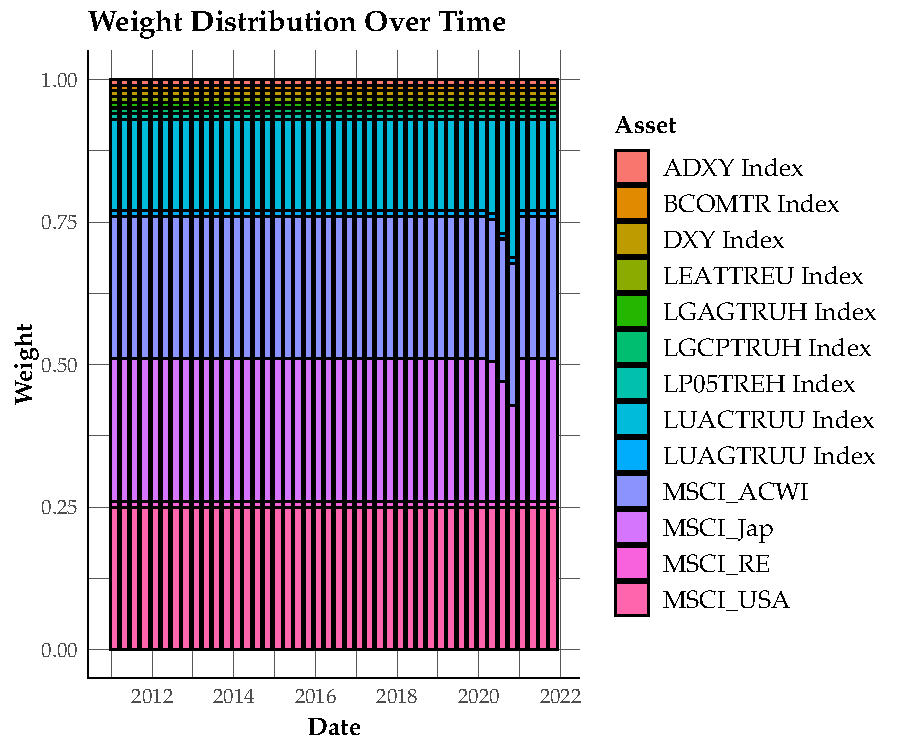
\includegraphics{Question-6_files/figure-latex/stacked-bar-1.pdf}

The figure above displays the weight distribution over time of various
assets within a portfolio. It is a stacked bar chart where each color
represents a different asset, and the combined weight of all assets adds
up to 1 (or 100\%) for any given period. This visual effectively
illustrates the changing allocation to each asset from 2012 through to
the beginning of 2022.

From the chart, we can observe that certain assets have maintained a
consistent presence in the portfolio over time, indicating a potentially
stable role in the investment strategy. On the other hand, some assets
show more variability in their allocation, which may reflect dynamic
adjustments to the portfolio in response to changing market conditions
or the rebalancing rules applied in the optimization process.

\hypertarget{correlation}{%
\subsection{Correlation}\label{correlation}}

The correlation plot presented here is a heat map that visualizes the
pairwise correlation coefficients between different financial indices.
Each square represents the correlation between the indices on the
vertical and horizontal axis.

In this plot:

\begin{itemize}
\tightlist
\item
  Red squares indicate a positive correlation, where the values closer
  to 1.0 suggest a stronger direct relationship.
\item
  Blue squares represent a negative correlation, with values closer to
  -1.0 indicating a stronger inverse relationship.
\item
  White or light-colored squares signify a neutral or no significant
  correlation, with values around 0.
\end{itemize}

Looking at the plot, we can see a mix of red and blue squares, which
implies a varied correlation structure within this set of indices. Some
indices, such as those along the diagonal, have a perfect positive
correlation with themselves, as expected. Others show varying degrees of
positive and negative correlations, indicating how some indices tend to
move together while others move in opposite directions.

The correlation plot reveals various degrees of relationships between
the indices:

\begin{itemize}
\tightlist
\item
  The \textbf{MSCI\_USA} and \textbf{MSCI\_ACWI} are highly correlated,
  as indicated by the dark red color, suggesting that movements in the
  US market have a strong influence on the global index.
\item
  Conversely, \textbf{DXY\_Index}, representing the US dollar index,
  shows a strong negative correlation (dark blue) with
  \textbf{BCOMTR\_Index}, an index representing commodities,
  highlighting an inverse relationship typically observed between the
  dollar and commodity prices.
\item
  The \textbf{LEATTREU\_Index} and \textbf{LGAGTRUH\_Index}, both
  related to fixed income, show a moderate to strong positive
  correlation with each other, visible in lighter red, implying that
  they may respond similarly to changes in interest rates or other
  economic factors affecting bonds.
\item
  The \textbf{MSCI\_Jap}, representing the Japanese market, displays a
  mix of correlations with global indices, with some reds indicating
  positive correlations and some blues indicating negative correlations,
  reflecting a more complex relationship influenced by specific regional
  economic events and global market trends.
\item
  The \textbf{MSCI\_RE}, reflecting real estate securities, seems to be
  less correlated (white to light blue) with bond indices like
  \textbf{LP05TREH\_Index} and \textbf{LUACTRUU\_Index}, suggesting that
  real estate securities may not always move in concert with bond
  markets, offering potential diversification benefits.
\end{itemize}

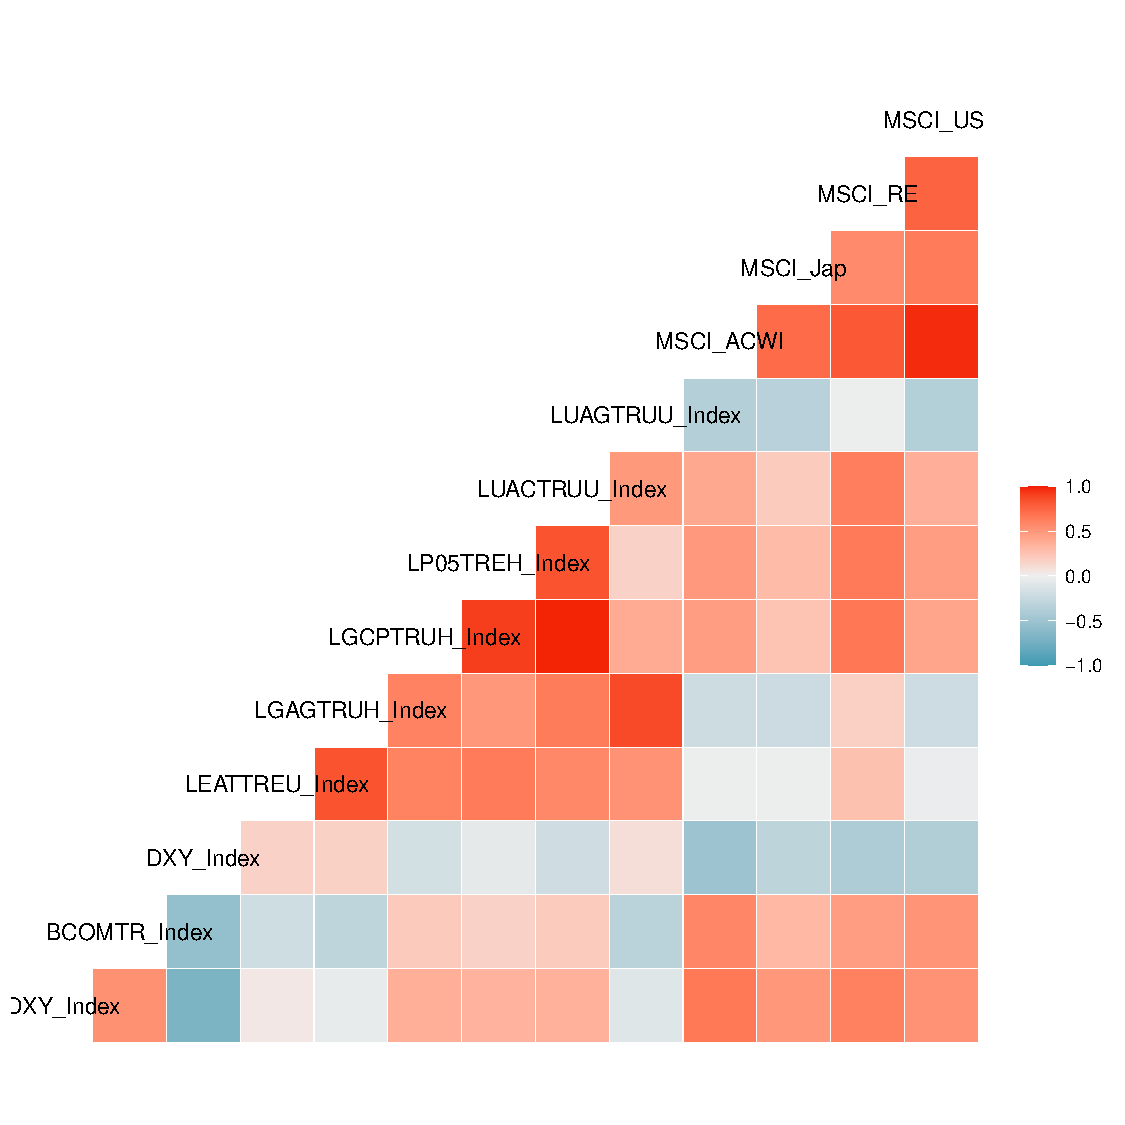
\includegraphics{Question-6_files/figure-latex/corrplot-1.pdf}

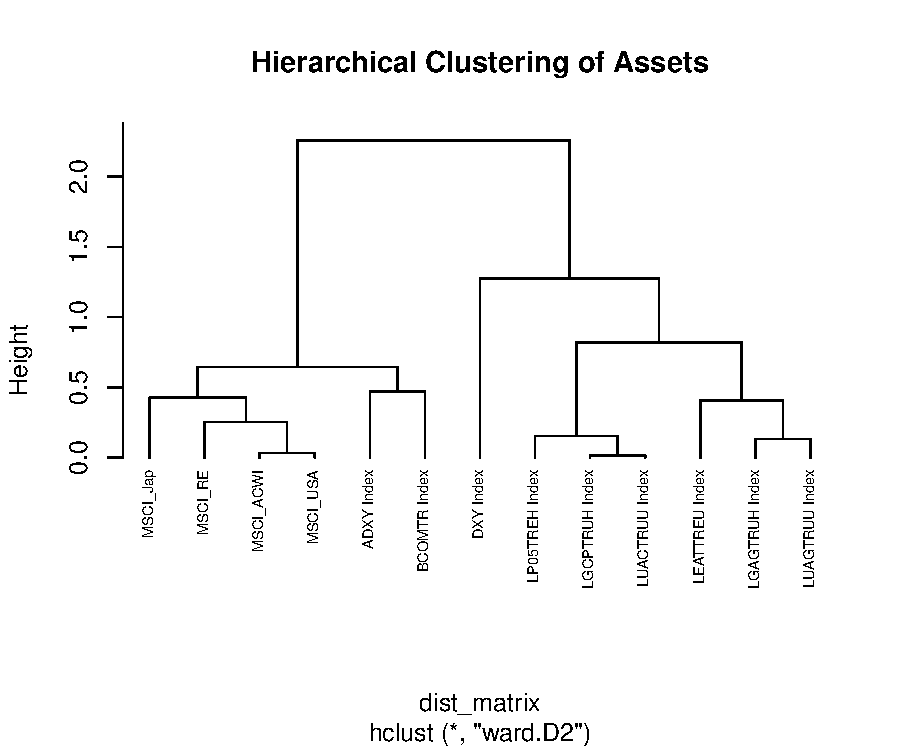
\includegraphics{Question-6_files/figure-latex/dendro-1.pdf}

\hypertarget{hierarchical-clustering}{%
\subsection{Hierarchical Clustering}\label{hierarchical-clustering}}

The dendrogram represents the hierarchical clustering of various
financial assets based on the similarity of their movements:

\begin{itemize}
\item
  \textbf{Close Clusters}: Assets that are grouped together at the lower
  heights (short vertical lines) are more similar to each other. For
  example, the \textbf{MSCI\_Jap} and \textbf{MSCI\_RE} are closely
  linked, suggesting that they have moved in a similar fashion
  historically. The \textbf{MSCI\_ACWI} and \textbf{MSCI\_USA} also form
  a close cluster, implying that global market movements are closely
  tied to US market movements.
\item
  \textbf{Distinct Groups}: On the right side of the dendrogram, there's
  a distinct grouping of bond indices such as \textbf{LEATTREU\_Index},
  \textbf{LGAGTRUH\_Index}, and \textbf{LUAGTRUU\_Index}, indicating
  that these assets share similar return patterns, likely reflecting
  similar market influences or investor behaviors.
\item
  \textbf{Height of Mergers}: The height at which clusters join
  represents the dissimilarity between groups. For example, the
  \textbf{ADXY Index} and the \textbf{BCOMTR Index} join at a higher
  level with the \textbf{DXY Index}, suggesting less similarity compared
  to other clusters.
\item
  \textbf{Diversification Insight}: The dendrogram can also be
  interpreted from a diversification perspective, where assets that do
  not cluster tightly with others (e.g., \textbf{DXY Index}) might
  provide diversification benefits to a portfolio that includes any of
  the closely linked assets.
\end{itemize}

\hypertarget{conclusion}{%
\section{Conclusion}\label{conclusion}}

The Global Balanced Index Fund portfolio, as analyzed and visualized
through the Lookback24 table and various plots, demonstrates a strategic
and responsive asset allocation. The portfolio benefits from a
disciplined approach to diversification, striking a balance between
fixed income and equities, and capturing growth opportunities in key
markets such as the United States and Japan. The optimizations reflect a
robust methodology that considers historical performance and aims for a
balanced risk-return profile, making it a viable and thoughtfully
composed investment vehicle.

\bibliography{Tex/ref}





\end{document}
